\documentclass[12pt, a4paper]{article}
\usepackage[italian]{babel}
\newcommand{\bigsize}{\fontsize{35pt}{20pt}\selectfont}
\newcommand{\mediumsize}{\fontsize{30pt}{20pt}\selectfont}
\newcommand{\normsize}{\fontsize{15pt}{10pt}\selectfont}
\usepackage{graphicx,float}
\usepackage[utf8]{inputenc}
%\usepackage[T1]{fontenc}


\begin{document}

\begin{titlepage}
\centering
		{\bigsize RELAZIONE PROGETTO\\}
		\vspace*{10px}
		{\bigsize PROGRAMMAZIONE\\}
		\vspace*{10px}
		{\bigsize AD OGGETTI\\}
		\vspace*{25px}
		
		{\bigsize Nome del progetto: \emph{QFit} \\}
		\vspace*{10px}
		



\includegraphics[scale=0.40]{img/logoProg.png}

		\vspace{20px}
		{\mediumsize Victor Dutca\\}
		\vspace*{5px}
		{\normsize Matricola: 1122137}
		\vspace*{30px}

		{\mediumsize  Laurea in Informatica\\ }
		\vspace*{30px}
		\centering
		
\includegraphics[scale=0.15]{img/logoMath.png}\\		
		\vspace*{\fill}
		{\normsize Anno Accademico 2019/2020\\ }
\end{titlepage}
\tableofcontents
\newpage

\section{Ambiente di sviluppo}
\vspace{10px}
\begin{itemize}
\item Sistema operativo
\begin{itemize}
	\item Ubuntu GNU\textbackslash Linux 19.04
\end{itemize}	
	\item Compilatore
	\begin{itemize}
		\item Ubuntu: \emph{g++}  \texttt{8.3.0} 
	\end{itemize}
	\item Versione Qt: 5.5.
\end{itemize}

\section{Scopo del progetto}
L'applicazione \emph{QFit} permette all'utente di inserire e tenere traccia dei propri allenamenti che possono essere di quattro tipologie: 
\begin{itemize}
\item Corsa
\item Ciclismo
\item Nuoto
\item Triathlon
\end{itemize}

Una volta inseriti i dati relativi a ciascun allenamento l'utente visualizza le calorie consumate durante e la quantità dei grassi bruciati durante tutto lasso di tempo indicato.
L'applicativo permette seguentemente di modificare l'allenamento, visualizzare i dati rispettivi all'allenamento e infine eliminarlo.
Il tutto avviene tramite lettura e scrittura da file \emph{.xml}.
Il programma fa uso di un contenitore templetizzato \emph{Dlista \textless Workout \textgreater}.
\newpage
\section{Gerarchie utilizzate}
Sono presenti due tipi di gerarchie per la parte logica e grafica rispettivamente.
\subsection{Gerarchia della logica}

\begin{figure}[H]
	\centering
	
	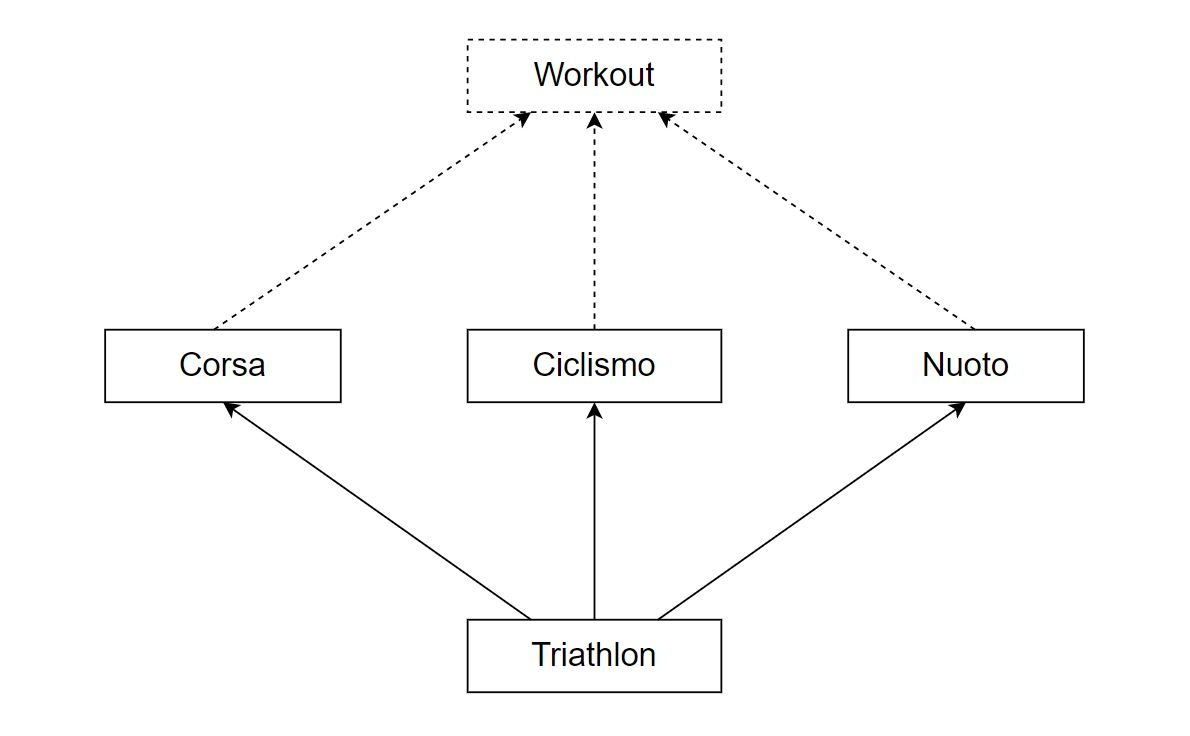
\includegraphics[scale=0.45]{img/graph.jpg}
	\caption{Gerarchia parte logica}
\end{figure}


\emph{Workout} è la classe base virtuale astratta la quale  da forma ad un generico allenamento inserito dall'utente tenendo conto della durata di quest'ultimo. In base alla durata vengono concretizzati tutti agli altri allenamenti mediante la definizione dei seguenti metodi virtuali:
\vspace{1cm}
\begin{itemize}
\item \textbf{\textasciitilde Workout() = default;}
\item \textbf{unsigned int GrassiBruc( ) const =0;}
\item \textbf{unsigned int calorie( ) const = 0;}
\item \textbf{bool operator==(const Workout \& ) const;}
\item \textbf{bool operator\textless =(const Workout \& ) const;}
\item \textbf{bool operator\textgreater =(const Workout \& ) const;}
\item \textbf{unsigned int get\_ durata() const;}
\item \textbf{void set\_ durata(unsigned int);}

\end{itemize}

Come menzionato in precedenza, dalla classe madre \emph{Workout} derivano le seguenti classi concretizzate: Ciclismo, Corsa, Nuoto e Triathlon. Tutti metodi virtuali delle classe base vengono overridati ad eccezione del distruttore.\par
Il metodo \emph{GrassiBrucci()} indica la quantità di grassi bruciati durante lasso di tempo dell'allenamento.\par
Il metodo \emph{calorie()} calcola le calorie consumate dall'allenamento.
\section{Gerarchia della Vista}
\begin{figure}[H]
	\centering
	
	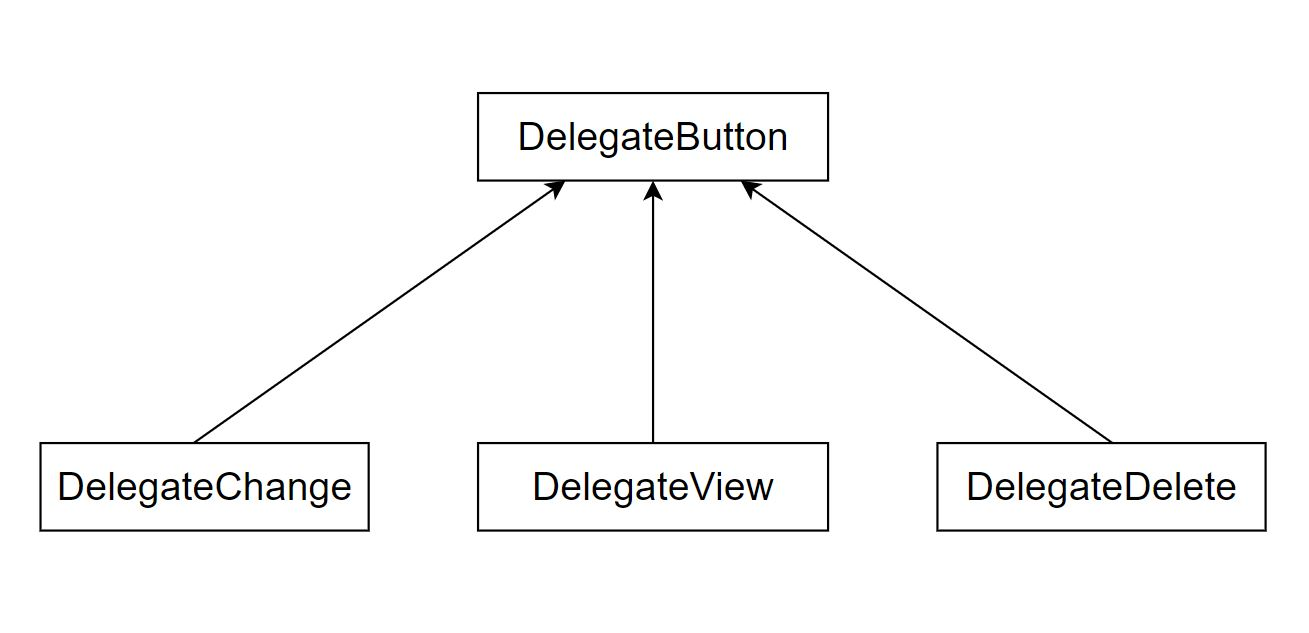
\includegraphics[scale=0.45]{img/viewGraph.jpg}
	\caption{Gerarchia parte logica}
\end{figure}
\emph{DelegateButton} è la classe base della gerarchia della vista la quale a sua volta è derivata da \emph{QItemDelegate} dalla quale i metodi \emph{paint()}, \emph{editorEvent()} e i distruttore sono overriddati  in \emph{DelegateButton}. Le sottoclassi derivate da \emph{DelegateButton} sono:
\begin{itemize}
\item[1)]\emph{DelegateView}:  gestisce l'input per la visualizzazione del record selezionato nella \emph{tableView} iniziale;
\item[2)]\emph{DelegateChange}: gestisce l'input per la modifica del record selezionato nella \emph{tableView} iniziale;
\item[3)]\emph{DelegateDelete}:  gestisce l'input per la cancellazione del record selezionato nella \emph{tableView} iniziale.
\end{itemize} 


\section{Utilizzo del codice polimorfo}

I metodi virtuali polimorfi della classe \emph{Workout} vengono chiamati nella seguente parte del codice:
\begin{itemize}
\item[\textgreater] \textbf{get\_ durata()}: linea 40 della classe \emph{ModelWorkout};
\item[\textgreater] \textbf{calorie()} linea 42 della classe \emph{ModelWorkout};
\item[\textgreater] \textbf{GrassiBruc()} linea 44 della classe \emph{ModelWorkout};
\item[\textgreater] \textbf{operator==} riga 119 della classe \emph{qfitciclismo};
\item[\textgreater] \textbf{operator==} linea 119 della classe \emph{qfitcorsa};
\item[\textgreater] \textbf{operator==} linea 109 della classe \emph{qfitnuoto};
\item[\textgreater] \textbf{operator==} linea 246 della classe \emph{qfittriathlon}.
\end{itemize}
\section{Manuale utente}

\end{document}